%\mychapter{3}{methodology}

\section{Current Project}

\subsection{Our framework}

We propose a method of pre-procesing spike times by looking at the time since the 
previous spike, which we refer to as the previous time. 
We smooth the previous time using the Laplace kernel
and then use the diffusion distance \cite{coifman2006diffusion} as a measure of similarity between smoothed previous time vectors. The low dimensional model is obtained by non-linear dimensionality reduction using the diffusion maps algorithm. The measure of ``goodness" of our low dimensional model is done by comparing the mutual information  \cite{quiroga2009extracting, Dayan2001}  between the resultant eigen vectors and and the position of the animal. We test our results using both simulations and behavioral real-world data.\\

A mathematical model based on the point-process framework is an appropriate approach for modeling  data from the CA1 region of the rat hippocampus for two reasons.
First, the position of the animal is coded by place cells using both the firing rate and the precise time at which the cells fire with respect to the hippocampal theta rhythm.
The theta rhythm is a sinusoid of frequency 7-12 Hz which occurs whenever a rat changes position in  a specific direction \cite{OKeefe1971, Burgess1993}.
Second,  metrics based on the point-process viewpoint are often non-Euclidean \cite{Aronov2004, Victor2005}. Moreover, there are specific examples like sensory space in  the olfactory system and the perceptual space of color vision which are typically non-Euclidean and analysis in the point-process framework would be most appropriate.\\


\subsection{Nature of our raw real-world data}
The raw data is a set of multiple single-unit single-trial spike trains,\\
\[ 
\text{T}^{\text{spike}} = \displaystyle \{ \{ t_{i}^{j} \} , 1 \leq i \leq n_{i}, 1 \leq j \leq 32 \}  
\]
recorded from 32 neurons, called  place cells, in the CA1 region of the rat hippocampus, where,
$\displaystyle  \{t_{i}^{j}\} =  \{t_{1}^{j}, ....., t_{n_{i}}^{j} \} $, represents  a sequences of n$_{i}$ recorded times at which the spikes of the j$^{th}$ neuron occurred.
The spike trains are of different lengths, n$_{i}$, where t$_{i}^{j}$ represents the i$^{th}$ spike time of the $j^{th}$ neuron.

\subsubsection{Preprocessing raw spike train data}
We pre-process the raw spike trains using two methods:
In the first method, the raw spike trains are smoothed with a Gaussian kernel to obtain the firing rate, as outlined in section 3.1. In the second method, we compute the time since the previous spike, which we refer to as, the \textit{previous time}. We then smooth the previous time with the Laplace Kernel,
to obtain a smoothed previous time function.\\


\subsubsection{Conversation to a firing rate}
For each neuron labeled j,  we convert the corresponding spike train
T$^{\text{spike}}_{j}(t) = \displaystyle \sum_{i=1}^{n_{i}} \delta(t-t_{i}^{j})$ (as in section 3.1), to obtain the firing rate function,
 R$^{j}$(t), by replacing, K in \eqref{firerate}, with the  Gaussian Kernel,\\
 K(t) =  $\displaystyle \frac{1}{\sigma \sqrt{2\pi}} e^{-\frac{t^2}{2\sigma^2}} $.
Thus, the firing rate function, for the j$^{th}$ neuron is given by

\begin{equation} \label{jfirerate}
\text{R}^{j}(t) = \sum_{i=1}^{n_{i}}  \frac{1}{\sigma \sqrt{2\pi}} 
e^{-\dfrac{(t_{i_{k}}^{j}  - t_{i_{l}}^{j})^2}{2\sigma^2}} 
\end{equation}

\subsubsection{The previous time function}
Given any time t, define the previous time of the $j^{th}$ neuron, denoted, $\text{P}^{j}(t)$, as follows: Let 
\[
t^{\text{spike}}_{\text{prev}}(t) = \displaystyle \max  \{  t^{j}_{i} \ \ | \ \ t^{j}_{i} < t, 1 \leq i \leq n_{i}, 1 \leq j \leq 32 \},\ \ \text{for all spike trains}, \quad  \{t^{j}_{i}\} \in T^{\text{spike}}
\]
The previous time function, P$^{j}(t)$, is given by, 
\begin{equation}\label{prevtimefun}
\text{P}^{j}(t) = t - t^{\text{spike}}_{\text{prev}}.
\end{equation}


See an example \eqref{ex1} below, illustrating how the previous time vectors are obtained.\\


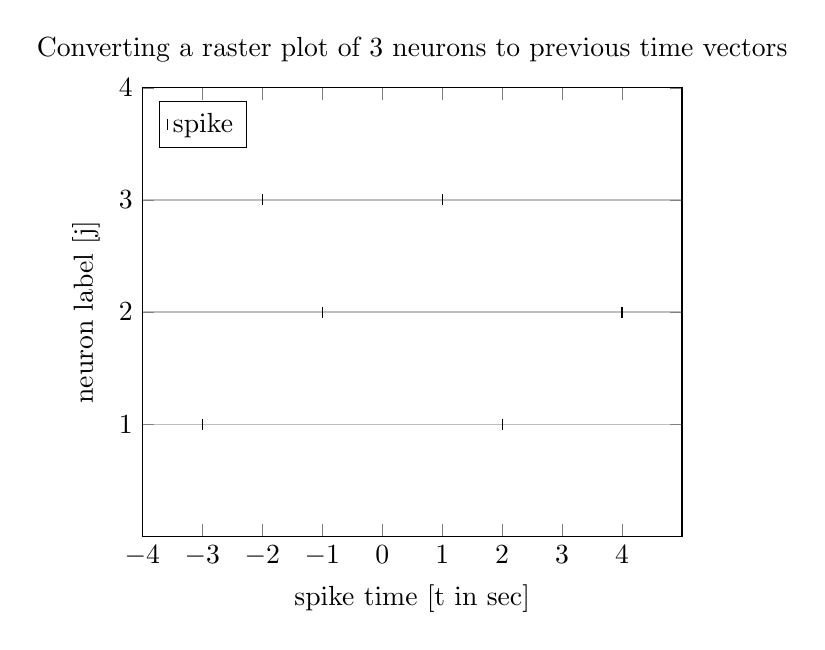
\begin{tikzpicture}
\begin{axis}[
    title={Converting a raster plot of 3 neurons to previous time vectors},
    xlabel={spike time [t in sec]},
    ylabel={neuron label [j]},
    xmin=-4, xmax=5,
    ymin=0, ymax= 4,
    xtick={-4, -3,-2,-1,0,1,2,3,4},
    ytick={1,2,3,4},
    legend pos=north west,
    ymajorgrids=true,
    grid style= solid,
]
 
\addplot[
    color=black,
    only marks,
    mark = |
    ]
    coordinates {
    (-3, 1)(-1,2)(-2, 3)(1, 3)(2,1)(4,2)
    };
    \legend{spike}
 
\end{axis}
\end{tikzpicture}


\begin{Ex}\label{ex1}

\[ \text{P}^{j}(0) =  \begin{cases} 
      3 & \text{if} \quad j=1 \\
      1 & \text{if} \quad j=2 \\
      2 & \text{if} \quad  j=3
   \end{cases}
\]


\quad

\[ \text{P}^{j}(2) =  \begin{cases} 
      5 & \text{if} \quad j=1 \\
      3 & \text{if} \quad j=2 \\
      1 & \text{if} \quad j=3
   \end{cases}
\]

add a pictures of conversion from raster plot to previous time. 
  
  
\end{Ex}


\subsubsection{Specific implementation}
We consider a population of, N$=32$, sensory neurons (place cells) encoding a 
one-dimensional circular stimulus variable, $\theta(t)$, which represents 
the position of the animal (rat), at any time, t, along a circular track, during
a behavioral task.
We let $\theta(t) = c t \ \ (\text{mod} \ \ 2\pi)$, where time, $t$, is in seconds,
$c = \dfrac{2\pi}{T_{\text{lap}}}$, is the speed of the animal, and
,$\text{T}_{\text{lap}}$, is the time taken for the animal to make one lap around the circle.
For this synthetic experiment, we assume that information about the animal's
environment is encoded by both the firing rate, $\text{R}^{j}(t)$,
and the precise time, $t$, at which individual spikes within a given time window
$(t, t+\Delta t)$, occurred.
We model the place field of the j$^{th}$ neuron using a sum of two Gaussians
\begin{equation}
{g}^{j}(\theta) = \displaystyle  f_{\text{bg}} + \sum_{j=1}^{2} f_{j} 
\exp\bigg(-\dfrac{\text{dist}^{2}(\theta - \phi_{j})}{2\sigma_{j}^{2}} \bigg)
\end{equation}
where, $f_{bg}$, is the background firing rate that is independent of the underlying stimulus, $f_{j}, j=1,2$ denote the maximum firing rates of each 
Gaussian,  $\phi_{j}$, is the preferred position of the j$^{th}$ 
neuron or the center of the j$^{th}$ place field.
Given any two angles, $\theta_{1}, \theta_{2} \in [0, 2\pi]$, the quantity
$\text{dist}(\theta_{1}, \theta_{2})$, denotes the shortest distance between 
two points on a unit circle, given by
\[
\text{dist}(\theta_{1}, \theta_{2}) = \big( \big( [\theta_{1} - \theta_{2}] + \pi  \big) \ \ \text{mod} \ \ 2\pi \big) - \pi.
\]
The experiment consists of a single trial, in which the spike train of the, j$^{th}$, neuron is generated according to approximately, a non-homogeneous poisson process, with firing rate, $R^{j}(t)$, defined by, $R^{j}(t) = g^{j}(\theta(t))$ in the interval $[0, T]$. Choosing m time points and setting the step size $\Delta t = \dfrac{\text{T}}{m}$, we subdivide the interval, [0, T], into short sub intervals [t$_{i}$, t$_{i} + \Delta t$] where $t_{i} = i \Delta t$, and generate
a spike with probability of $\text{R}^{j}(t)\Delta t << 1$, otherwise no spike is generated.  We then sample the brain state uniformly at random, at these times $t_{i}$, to obtain the firing rate and previous time data. For each time $t_{i}$, we sample from  \eqref{jfirerate} and  \eqref{prevtimefun}, to obtain the firing rate vectors 
\[ \vect{r}(t_{i}) = (r^{1}(t_{i}), r^{2}(t_{i}), \ldots, r^{N}(t_{i}))^{\top},
\]
and previous time vectors
\[
\vect{p}(t_{i}) = (p^{1}(t_{i}), p^{2}(t_{i}), \ldots, p^{N}(t_{i}))^{\top},
\] respectively.
Thus at each time, $t_{i} \in [0,T]$, the position of the animal, $\theta(t_{i})$, is associated with a previous time vector, $\vect{p}(t_{i})$,
and a firing rate vector, $\vect{r}(t_{i})$.
These vectors are our data points.  Here, N=32 since we are analyzing data from 32 single-unit recordings. 



\subsection{Distance measure used in results section}
Given two time points $t_{1}$ and $t_{2}$ representing different brains, we form 
the corresponding previous time vectors $\vect{p}(t_{1})= (p^{1}(t_{1}), p^{2}(t_{1}), \ldots, p^{32}(t_{1}))^{\top} $  and  $\vect{p}(t_{2}) = (p^{1}(t_{2}), p^{2}(t_{2}), \ldots, p^{32}(t_{2}))^{\top}$ in $\R^{32}$.

We use the l$_{1}$ norm, d, to compute the distance between the two vectors:

\begin{equation}\label{distPrevtime}
\text{d}(\vect{p}(t_{1}), \vect{p}(t_{2}) ) = 
\displaystyle \sum_{i=1}^{32} \abs{ p^{i}(t_{1}) - p^{i}(t_{2})   }
\end{equation}

Similarly, we use the l$_{1}$ norm to compute the distance between two firing rate vectors:

\begin{equation}\label{distFirerate}
\text{d}(\vect{r}(t_{1}), \vect{r}(t_{2}) ) = 
\displaystyle \sum_{i=1}^{32} \abs{ r^{i}(t_{1}) - r^{i}(t_{2})   }
\end{equation}


\subsubsection{Similarity measure used in results section}
We form pair-wise similarities, $s_{ij}$, between each data point
using the Gaussian kernel 
\[
s_{ij} = e^{-\dfrac{\text{dist}^{2}(\vect{x}_{i}, \vect{x}_{j})}{2\sigma^2}} 
\]
where $\text{dist}(\vect{x}_{i}, \vect{x}_{j})$ is given by equations
\eqref{distPrevtime} and \eqref{distFirerate}.
We then apply diffusion maps to the resultant similarity matrix S = (s$_{ij}$) 
as described in section 3.6.6, to obtain a low dimensional model for the 
firing rate and previous time data.
The two parameters in diffusion maps are $\sigma$ and $\alpha$.
We set $\sigma =1$ and $\alpha = 0.5$ for both the synthetic and real-world data.























%\begin{itemize}

%========suggested by Duane=========================================
%\item  First mention that there is a general conceptual framework
%namely dimensionality reduction and then say that
% the metric a approach is just one of the ways of doing dim reduction
% yet ensuring minimal information loss.

%\item The previous/next time approach is our new way of preprocessing
% the data and then using some of the usual metrics to analyze it.

%============end suggestion=========================================
%\item How did you create the metric and what precisely is it's definition?
%\item Experimental design. Discuss how the data was collected using a diagram
%\item Mention that this kind of analysis has never been 
%applied to this Redish Lab data.
%\item describe your methodology starting with the fake brain model and then tests on real data
%\item what are the names and definitions of the algorithms you're using?
%\item what is dimensionality reductions and why are you using linear instead of non linear
%\item Why did you choose this particular algorithm(s)?
%\item What is wrong with using PCA or Kernel PCA?
%
%\end{itemize}





